\documentclass[a4paper]{article}

\usepackage{cite}%多个文献引用
\usepackage{graphicx}
\usepackage{array}%调节表格行高
\usepackage{multirow,makecell}%多行表格
\usepackage{tabularx}%表格固定列宽
\usepackage{subfigure}
\usepackage{titlesec}%标题格式设置
\usepackage{amsmath}
\usepackage{amssymb}
\usepackage{tabularx}
\usepackage{makecell}
\usepackage{geometry}
\usepackage{float}
\usepackage{setspace}%行距包
\usepackage{siunitx}
\usepackage{mdwlist}
\usepackage{tabu}
\usepackage{enumerate}

\geometry{top=1.54cm,bottom=2.54cm,left=2.5cm,right=2.5cm}


\begin{document}
\begin{center}
\bf\Large
EE 105 Feedback Control Systems\par
Department of Electrical and Computer Engineering\par
Tufts University Fall 2018\par
Homework \#9\par   
\end{center}
\begin{table}[H]
\begin{center}
\begin{tabular*}{\textwidth}{@{\extracolsep{\fill}}lcr}
Name: {\it Shang Wang} &Student ID: {\it 1277417} &E-mail: {\it shang.wang@tufts.edu}\\
\hline
\end{tabular*}
\end{center}
\end{table}

% \begin{figure}[H]
% \centering
% 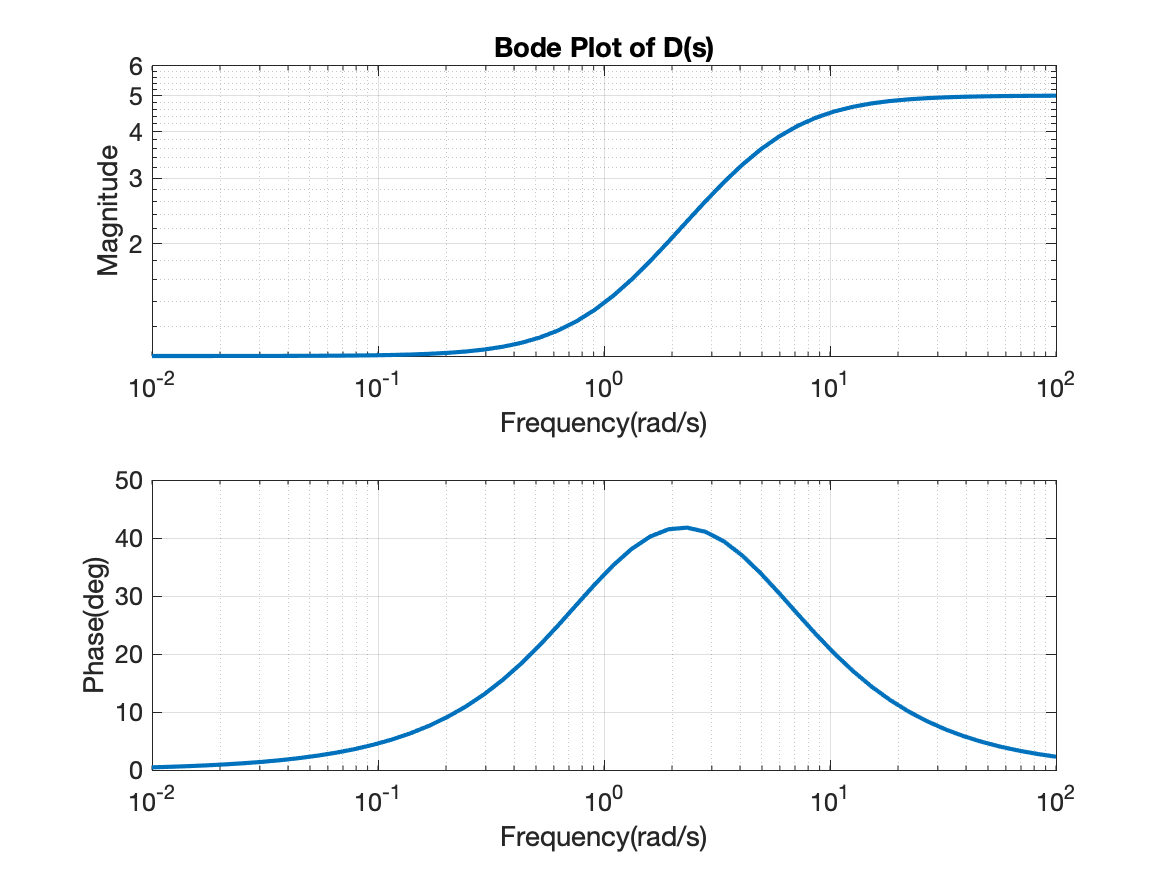
\includegraphics[width = 0.6\textwidth]{pic/0.png}
% \end{figure}



\section{Problem 1}
\subsection{Part A}
For ideal Op-Amp, 
$$
\frac{v_{out}}{v_{in}} = -\frac {Z_{out}}{Z_{in}}
$$
where
$$
Z_{in} = (\frac{1}{sC}+R_2)//R_1;\ \ Z_{out} = R_1
$$
So 
$$
D(s)  = - \frac{v_{out}}{v_{in}} = \frac{(R_1+R_2)s + 1}{ R_2C s + 1 }
$$
We have
$$
(R_1+R_2)C = \frac {1}{0.2}R_2C
$$
So I choose parameters
$$
R_1 = 80\ {\rm k\Omega }, \ \ R_2 = 20\ {\rm k\Omega }, \ \ C = 10\ {\rm \mu F}
$$
\subsection{Part B}
The bode plot of $D(s)$(after applying the unit inverter)
\begin{figure}[H]
\centering
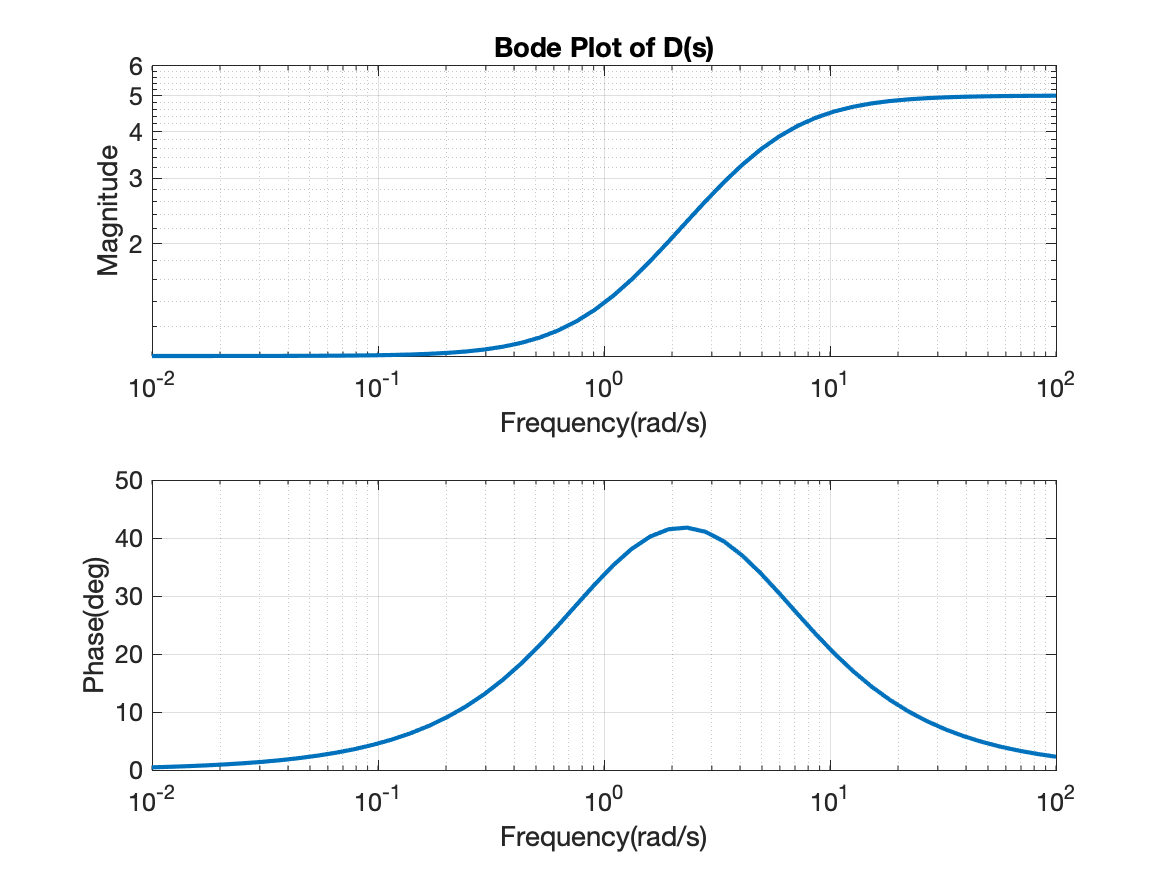
\includegraphics[width = 0.6\textwidth]{pic/0.png}
\end{figure}
\noindent We can see the turning point at about $\omega = 1$ and $5$. 

\subsection{Part C}
Say $V_m$ is the votage of the inverting input.
\begin{equation*} 
\left\{
\begin{aligned}
& V_{out} = -V_m\frac{A_0}{\tau s +1} \\
& V_m = V_{in} + \frac{Z_{in}}{Z_{in}+Z_{out}}(V_{out}-V_{in})
\end{aligned}
\right.
\end{equation*}
eliminate $V_m$, 
$$
\frac{V_{out}}{V_{in}} = -\frac{Z_{out}}{Z_{in}}\frac{A_0}{(\tau s +1 )(1 + \frac{Z_{out}}{Z_{in}})+ A_0} = -D(s)\frac{L(s)}{1+L(s)}
$$
where
$$
L(s) = \frac{A_0}{(\tau s + 1)(D(s)+1)} =  \frac{A_0}{2}\frac{\alpha s +1 }{(\tau s + 1)(\beta s+1)}
$$
In which,
$$
\alpha = R_2C, \ \ \beta = (\frac{R_1}{2}+R_2)C
$$
\subsection{Part D}
Substitute these quantity into $L(s)$,
$$
L(s) = \frac{20000 s + 100000}{0.03 s^2 + 0.65 s + 1}
$$
The bode plot,
\begin{figure}[H]
\centering
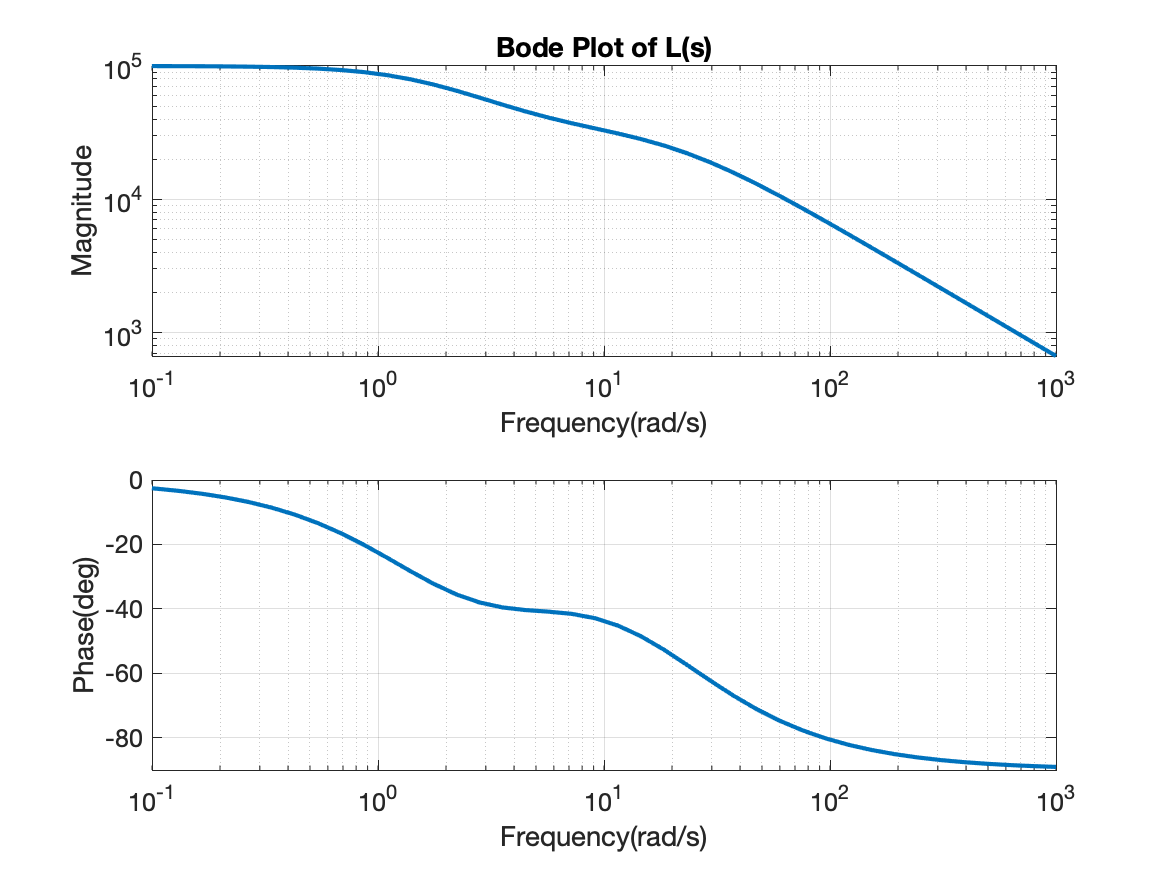
\includegraphics[width = 0.6\textwidth]{pic/1.png}
\end{figure}
\noindent And the Nyquist plot,
\begin{figure}[H]
\centering
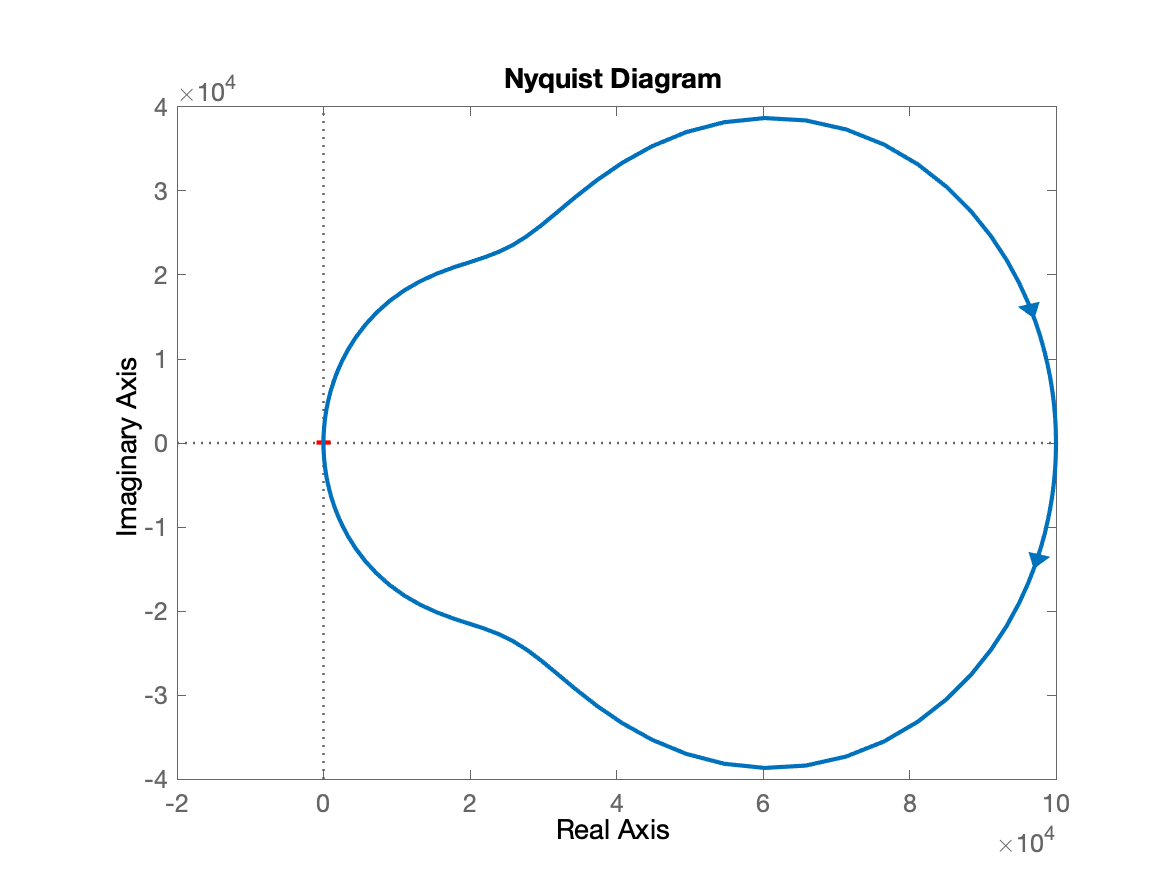
\includegraphics[width = 0.6\textwidth]{pic/2.png}
\end{figure}

\subsection{Part E}
According to the Bode plot, the phase of $L(s)$ will never be lower than 90 degree. So the close loop system is stable.







\end{document}